\documentclass[
	english,
	fontsize=10pt,
	parskip=half,
	titlepage=true,
	DIV=12
]{scrartcl}

\usepackage[utf8]{inputenc}
\usepackage{babel}
\usepackage[T1]	{fontenc}
\usepackage{lmodern}
\usepackage{microtype}
\usepackage{color}
\usepackage{csquotes}
\usepackage{xspace}

\usepackage{hyperref}

\newcommand*{\tabcrlf}{\\ \hline}

\usepackage{amsmath}
\usepackage{amssymb}
\usepackage{dsfont}
\usepackage[arrowdel]{physics}
\usepackage{mathtools}
\usepackage{siunitx}

\usepackage{minted}
	\usemintedstyle{friendly}

\newcommand*{\inPy}[1]{\mintinline{python3}{#1}}
\newcommand*{\ie}{i.\,e.\xspace}
\newcommand*{\eg}{e.\,g.\xspace}

\begin{document}

\part*{Python Problems 05, Summer 2021}
In this exercise, we will write code that reads text data files from the hard disk, displays them as a plot on screen and allows to superimpose one or more fits onto that data. While you have seen the elementary ideas on how to do that in class, many details were not covered. This is by design: looking up things online is an essentail part of the day-to-day business of any programmer. I've put some links in the description below, but you might find it useful to use your search engine of choice every once in a while. In general, it is a good idea to search for terms matching the pattern \texttt{tkinter verb details}, \eg \texttt{tkinter set font color}. Usually, searching for English terms yields more and better results than trying to find resources in other languages.

The features to implement are rather extensive, but just see how far you get, and feel free to omit parts of this sheet. For example, you can leave out the Fourier analysis/synthesis part of this problem statement or drop the fit part alltogether.

Note that this could have been a valid final project code.

\section{Load File Dialog}
Familiarize yourself with the open file dialog as provided by the tkInter module. Read up on \url{https://tkdocs.com/tutorial/windows.html#dialogs}, then test what you've just found by writing a short code that allows the user to select a file from their hard disk. Print the selected filename on the console.

You can make it such that the dialog only shows files with certain extensions. For that, an optional argument \texttt{filetypes} can be passed to the function \texttt{askopenfilename}. This optional argument should hold a \inPy{list} of \inPy{tuple}s of \inPy{str}ings. Each \inPy{tuple} comprises of two strings, the first of them being a description for the user and the second one describing the file pattern. A file pattern is a string comprising \emph{wildcard} the character \texttt{*} (think of it as a joker) and any mandatory characters that should be filtered for. Example: \inPy{"*.py"} would be the file pattern that matches all files with the extension \texttt{py}.

Use this knowledge to adjust your code such that the resulting dialog allows the user to select CSV files (\texttt{*.csv}), Text files (\texttt{*.txt}) or Any files (\texttt{*}). The resulting dialog should look like this:
\begin{center}
	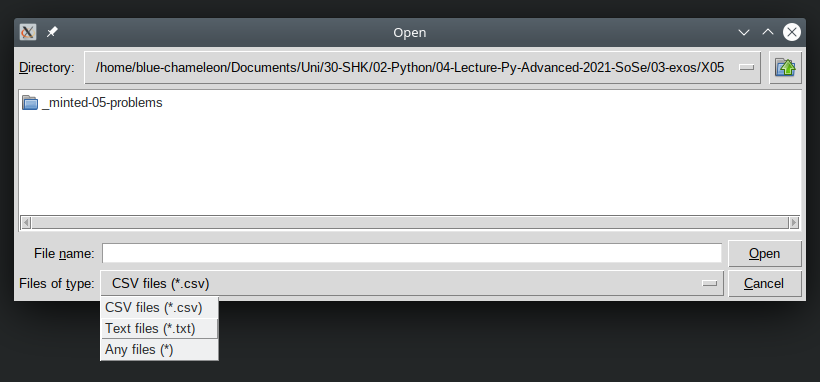
\includegraphics[width=.6\linewidth]{./tk-filepicker}
\end{center}

\section{Matplotlib in tkInter}
The search term \texttt{matplotlib in tkinter frame} leads to this ressource: \url{https://matplotlib.org/3.1.0/gallery/user_interfaces/embedding_in_tk_sgskip.html}
Read and understand the example shown there. Focus on the \texttt{canvas}, and forget about the \texttt{NavigationToolbar2Tk} and the \texttt{key\_press\_handler}.

Then generate a TK window with a button and a dummy MatPlotLib plot.

\section{Widgets Layout}
Now, generate the main window as shown below. For the time being, forget about what functions the buttons serve, but only try to write code that produces an user interface that looks as close as possible to the one shown on this problem sheet:
\begin{center}
	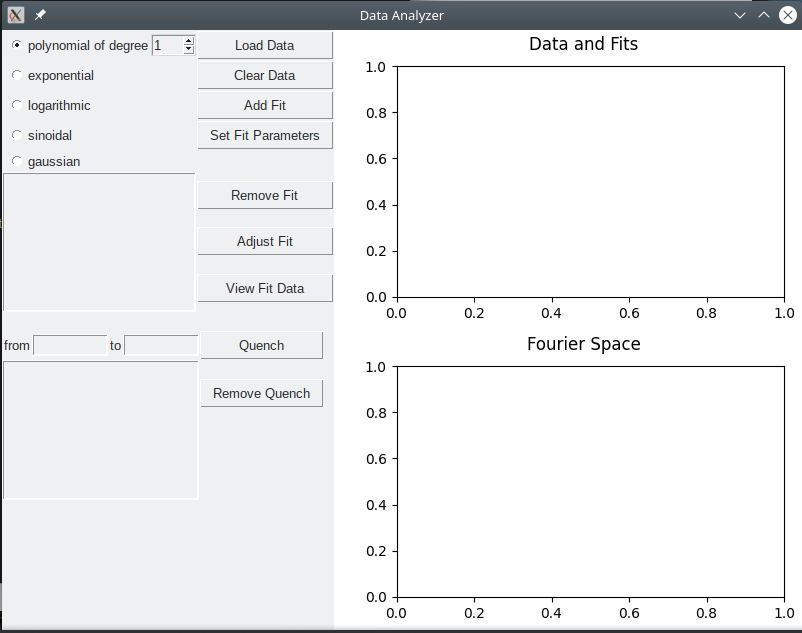
\includegraphics[width=.8\linewidth]{./tk-MainWin}
\end{center}
Note that the big boxes are Listboxes and the small boxes next to the labels "from" and "to" are Entries. The widget next to the Radiobutton "polynomial of degree" is a Spinbox.

\section{Data Structures}
Think now of how to represent the plot data in memory and where to instantiate them (\ie in which scope). You will need X- and Y-Data for the original data, as well as Frequency- and Intensity-Data for the Fourier spectrum.

Now make it such that clicking the button "Clear Data" erases all data in memory and resets the plot areas.

\emph{Hint:} The method \texttt{axesobject.cla()} restores a pristine drawing area.

\emph{Hint:} If you followed the example from task 2, the MatPlotLib figure has been \enquote{captured} by the TK system. Changes are not automatically rendered on screen. Instead, you'll need a call to \texttt{canvas.draw()} each time you want to make changes visible.

\emph{Hint:} You can add/change the function of a Button \emph{after} it has been created. To do so, use \texttt{handleToButton["command"] = function}.
\end{document}
